在分析后每个指标的统计分布情况后,发现有些变量的极差相差无几,甚至分布情况也大致相同,这里怀疑变量之间存在相关性,并进行相关性分析如下:

\begin{figure}[h!]
	\centering
	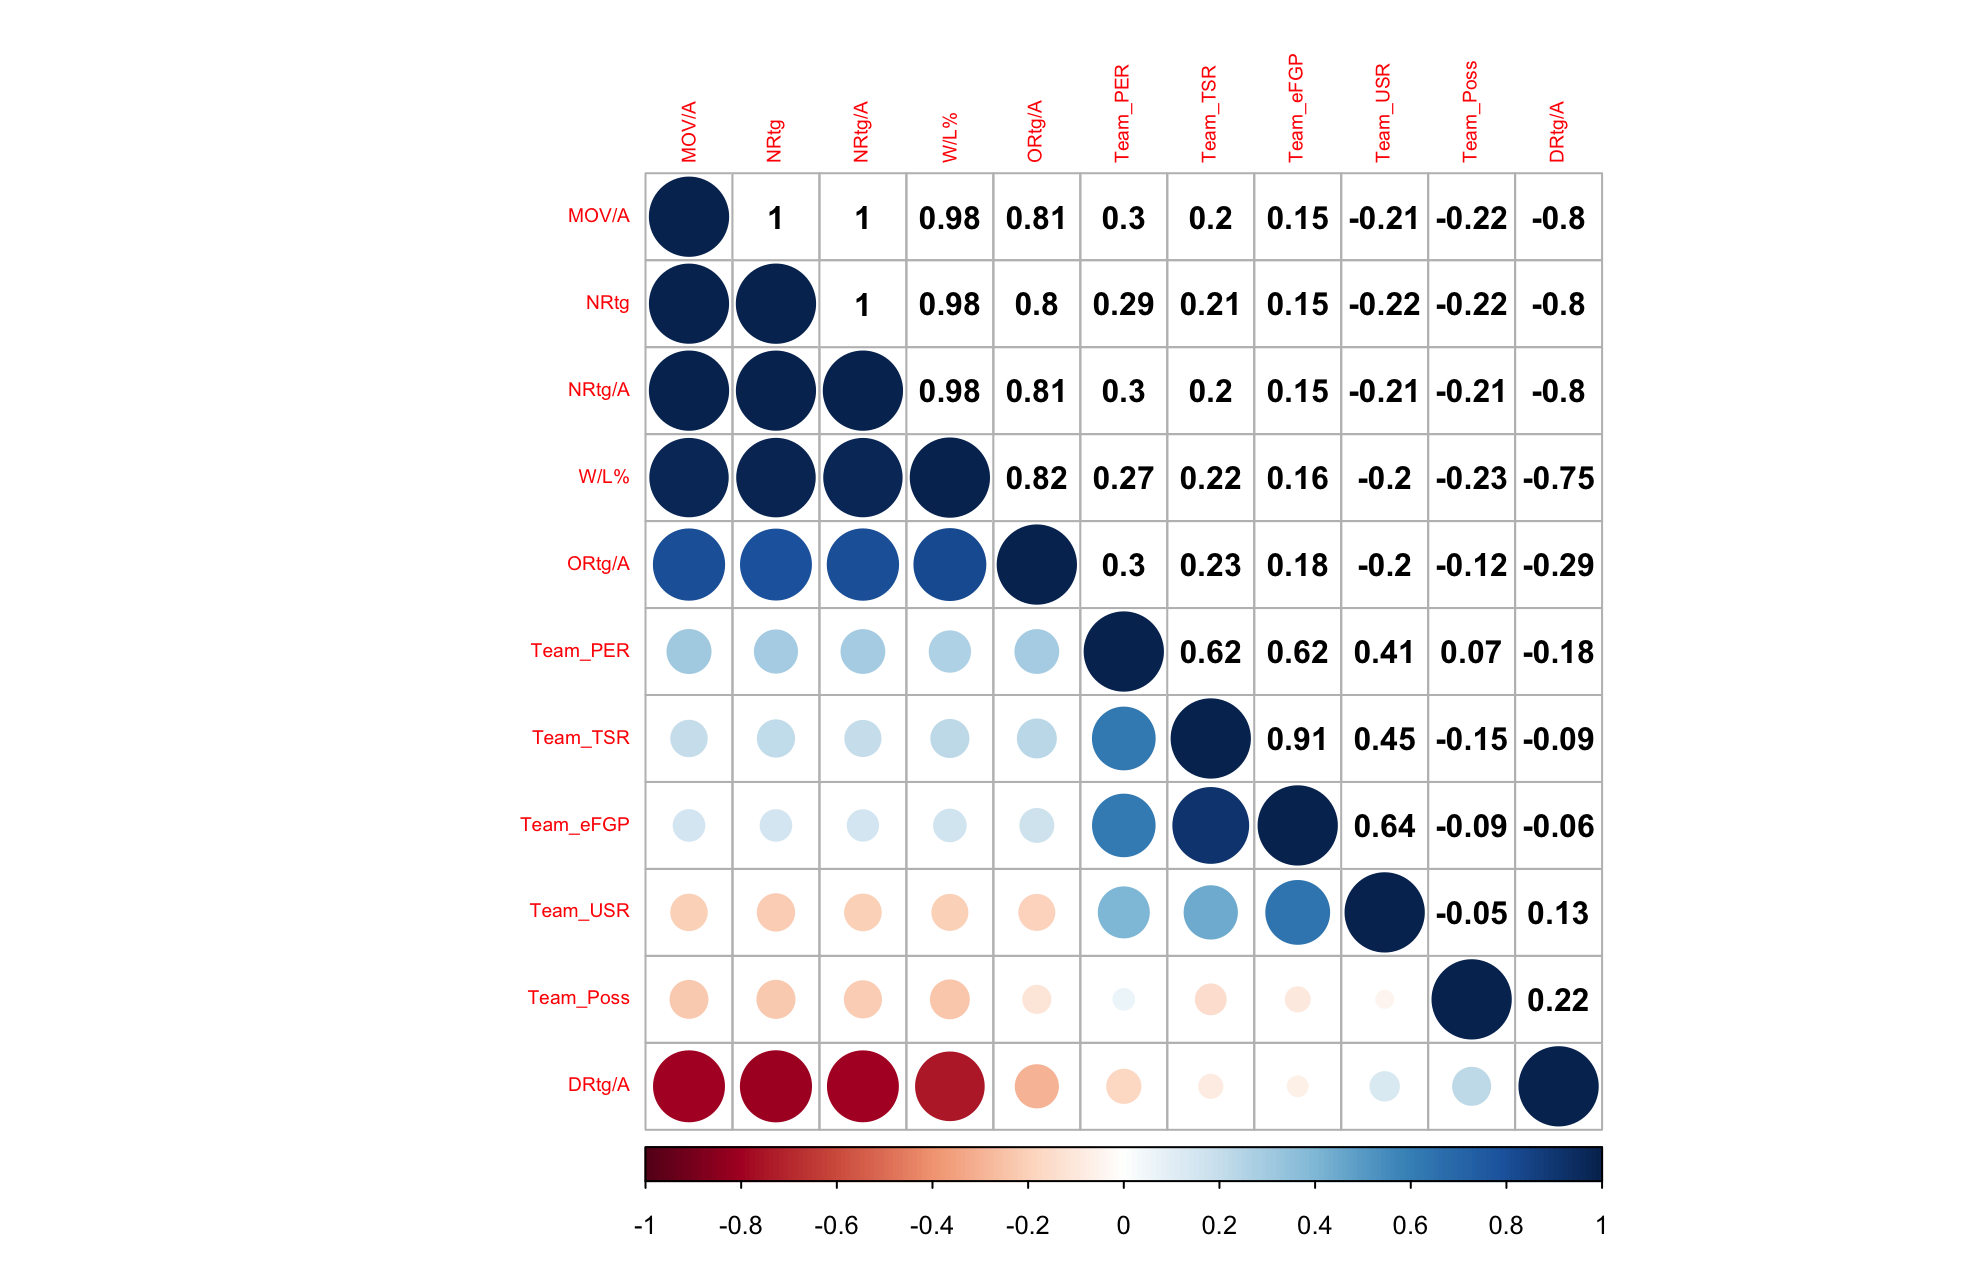
\includegraphics[width=15cm]{corr.png}\label{fig:16}
	\centering
	\caption{变量相关图}
\end{figure}

上图中蓝色代表变量之间有正相关,红色代表变量之间有负相关关系,蓝色越深面积越大说明变量之间的正相关关系越强,对角线是变量自身的相关性,是完全相关相关系数为1,但是净得分和比分差距与胜率之间有1的相关性,这里可以认为净得分和比分差距是完全共线性,可以认为这两个变量是相同的,剔除比分差距这个变量。胜率和净得分有0.98的高度相关性,说明球队净得分越高,则球队的胜率越高,由于两者相关性过高,在建模时容易覆盖其他变量对因变量的影响,所以去除净得分变量。球队进攻效率和胜率之间的相关性是0.81,说明进攻效率越高,球队获胜可能性越高,而防守效率与球队胜率之间有-0.8的相关性,即防守失分率越低,球队获胜可能性越高,防守失分率和进攻效率之间有-0.29的相关性,说明防守效率和进攻效率并不是很强的相关;球员效率与胜率有0.3的正相关性,说明球员效率越高,球队获胜的可能性越大;球员的利用率与胜率之间有0.27 的相关性,说明球员的利用率越高,球队获胜的可能性越大;球员利用率和球员的有效得分率之间有0.64的正相关,说明一个球员在控球时打出越高的有效得分说明球员的利用率越高。
\\

根据上述结论,我们剔除与胜率有极大相关性的变量,研究球队胜率W/L\%(因变量),球队攻击效率ORtg/A, 球队防守效率DRtg/A, 球队实际命中率Team\_TSR,,球队球员有效得分率Team\_eFGP,球队有效利用率Team\_USR,球队整体球员效率Team\_PER,球队控球次数Team\_Poss这8个变量对球队胜率的影响大小。
